\documentclass[12pt]{article}
\usepackage[utf8]{inputenc}
\usepackage[paperwidth=8.5in, paperheight=80in, margin=1.5in]{geometry}

\usepackage{graphicx}
\usepackage{amsmath}
\numberwithin{equation}{section}
\usepackage{titlesec}
\setcounter{secnumdepth}{4}
\pagenumbering{gobble} % removes page number from TOC and pages

% removes space between enumerate items
\usepackage{enumitem}
\setlist[enumerate]{itemsep=-1ex}

\usepackage{xcolor}
\definecolor{xlinkcolor}{cmyk}{1,1,0,0}
\usepackage[colorlinks,allcolors=xlinkcolor]{hyperref}

% remove dots in TOC
\usepackage[titles]{tocloft}
\renewcommand{\cftdot}{}

\setcounter{tocdepth}{2}

\title{Econometrics}
\author{Andrew Lu}
\date{Mr. Lizardo, Fall 2020}

\begin{document}

    \maketitle
    \label{sec:top}
    \tableofcontents

\section{Introduction to Statistics}

\subsection{Statistical Measures}
\subsubsection{Mean}
\begin{align}
    \mu=\frac{\sum\limits_{i=1}^{N}{x_i}}{N} \\
    \overline{X}=\frac{\sum\limits_{i=1}^{N}{x_i}}{n}
\end{align}

\subsubsection{Variance}
\begin{align}
    \sigma^2=\frac{\sum\limits_{i=1}^{N}{(x_1-\mu)^2}}{N} \\
    s^2=\frac{\sum\limits_{i=1}^{n}{(x_1-\Bar{x})^2}}{n-1}
\end{align}
where $\sigma^2=$ population variance and $s^2=$ sample variance. The denominator is $n-1$ for sample variance calculations because of degrees of freedom.

\subsubsection{Standard Deviation}
\begin{align}
    \sigma=\sqrt{\frac{\sum\limits_{i=1}^{N}{(x_1-\mu)^2}}{N}} \\
    s=\sqrt{\frac{\sum\limits_{i=1}^{n}{(x_1-\Bar{x})^2}}{n-1}}
\end{align}

\subsection{Data Distribution}
\subsubsection{Histograms}
\begin{figure}[!ht]
    \centering
    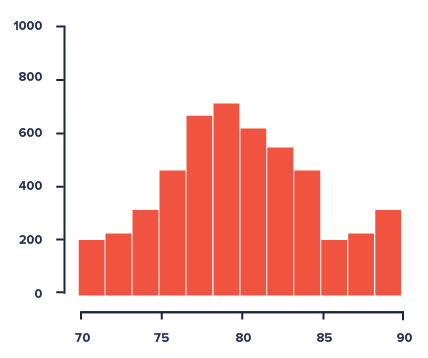
\includegraphics[width=0.6\linewidth]{figures/histogram.png}
\end{figure}

\subsubsection{Box Plots}
\begin{figure}[!ht]
    \centering
    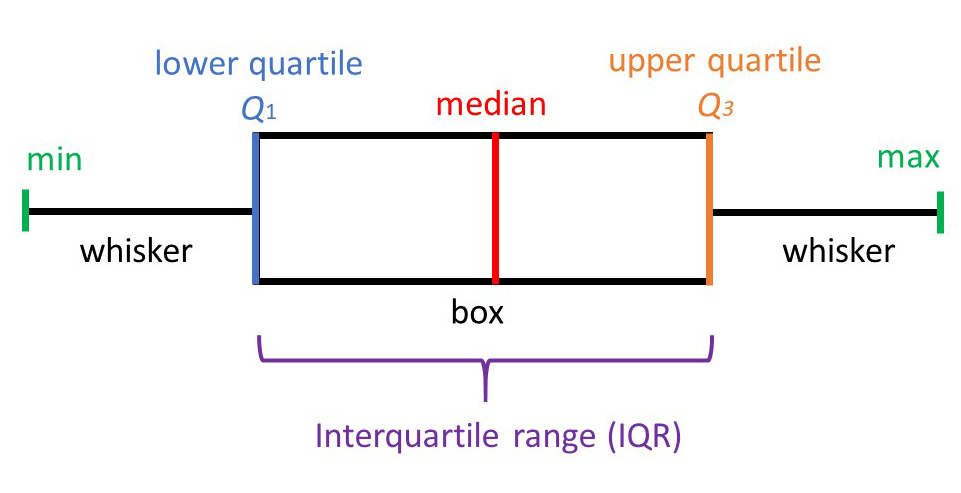
\includegraphics[width=0.8\linewidth]{figures/boxplot.jpg}
\end{figure}
Outliers: any value outside 1.5 $\times$ IQR above Q3 or below Q1
\begin{align}
    IQR = Q3 - Q1
\end{align}

\subsubsection{SOCS}
\begin{enumerate}
    \item Symmetry: positive/right skew, negative/left skew, or normal curve
    \item Outliers: skew the distribution in its direction
    \item Center: mean = balancing point, median = data split in half
    \item Spread: outliers affect spread by impacting skew
\end{enumerate}
\begin{figure}[!ht]
    \centering
    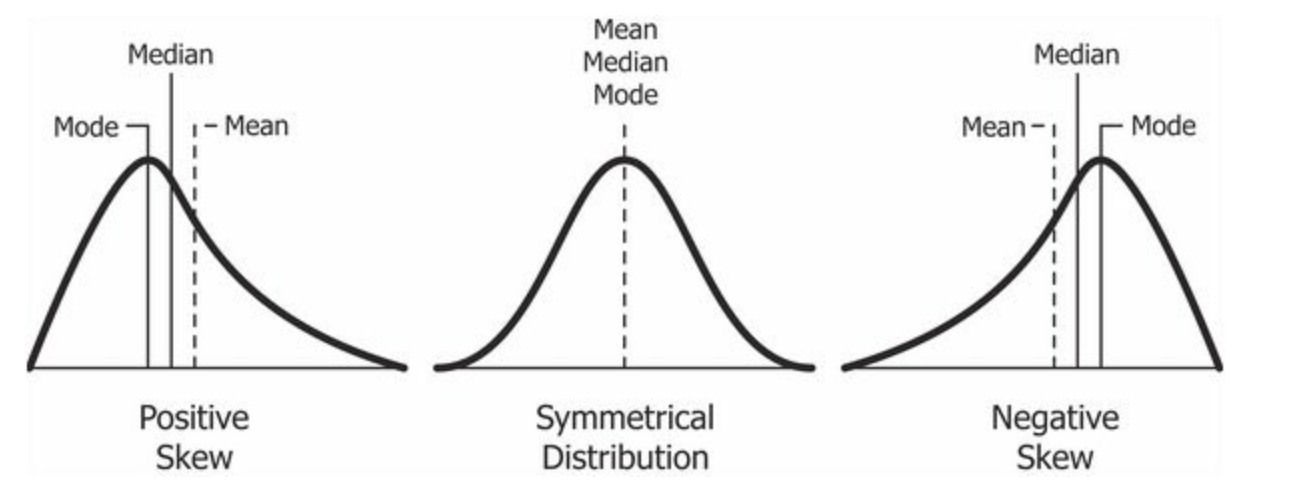
\includegraphics[width=0.9\linewidth]{figures/skew.png}
\end{figure}

\subsection{Probability}
\begin{enumerate}
    \item Conditional Probability:
    \begin{align}
        P(A|B) = \frac{P(A \cap B)}{P(B)}
    \end{align}
\end{enumerate}

\subsection{Discrete Random Variables}
\subsubsection{Measures}
\begin{gather}
    \mu_x = \sum x \times p(x) \\
    \sigma^2_x = (x_1-\mu_x)^2 p_1 + (x_2-\mu_x)^2 p_2 + ... + (x_i-\mu_x)^2 p_i
\end{gather}

\subsubsection{Binomial Situations}
\begin{enumerate}
    \item B: Binary Outcomes
    \item I: Independent Trials
    \item N: Number of Trials
    \item S: Success Probability
\end{enumerate}
\subsubsection{Binomial Probabilities}
\begin{gather}
    \mu_k = np \\
    P(k) = \binom{n}{k} p^k (1-p)^{n-k} \\
    \sigma = \sqrt{np(1-p)}
\end{gather}

\subsection{Continuous Random Variables}
%\subsubsection{Probability Density Function}
%\subsubsection{Area Under Curve (AUC)}
\subsubsection{Normal Distribution}
\begin{figure}[!ht]
    \centering
    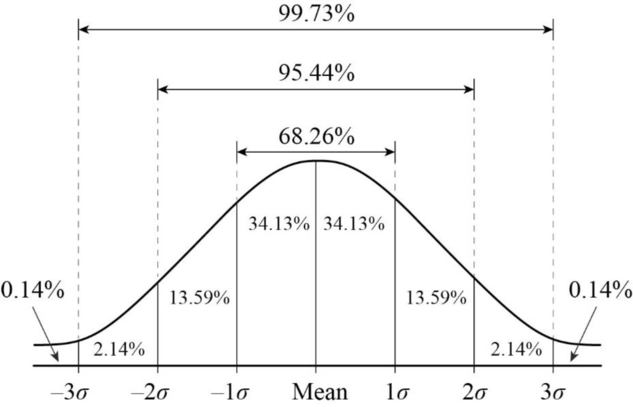
\includegraphics[width=0.8\linewidth]{figures/normalcurve.png}
\end{figure}

\subsubsection{Z-Score}
\begin{gather}
    \text{z-score: } z = \frac{x-\mu}{\sigma}
\end{gather}

% \begin{figure}[!ht]
%     \centering
%     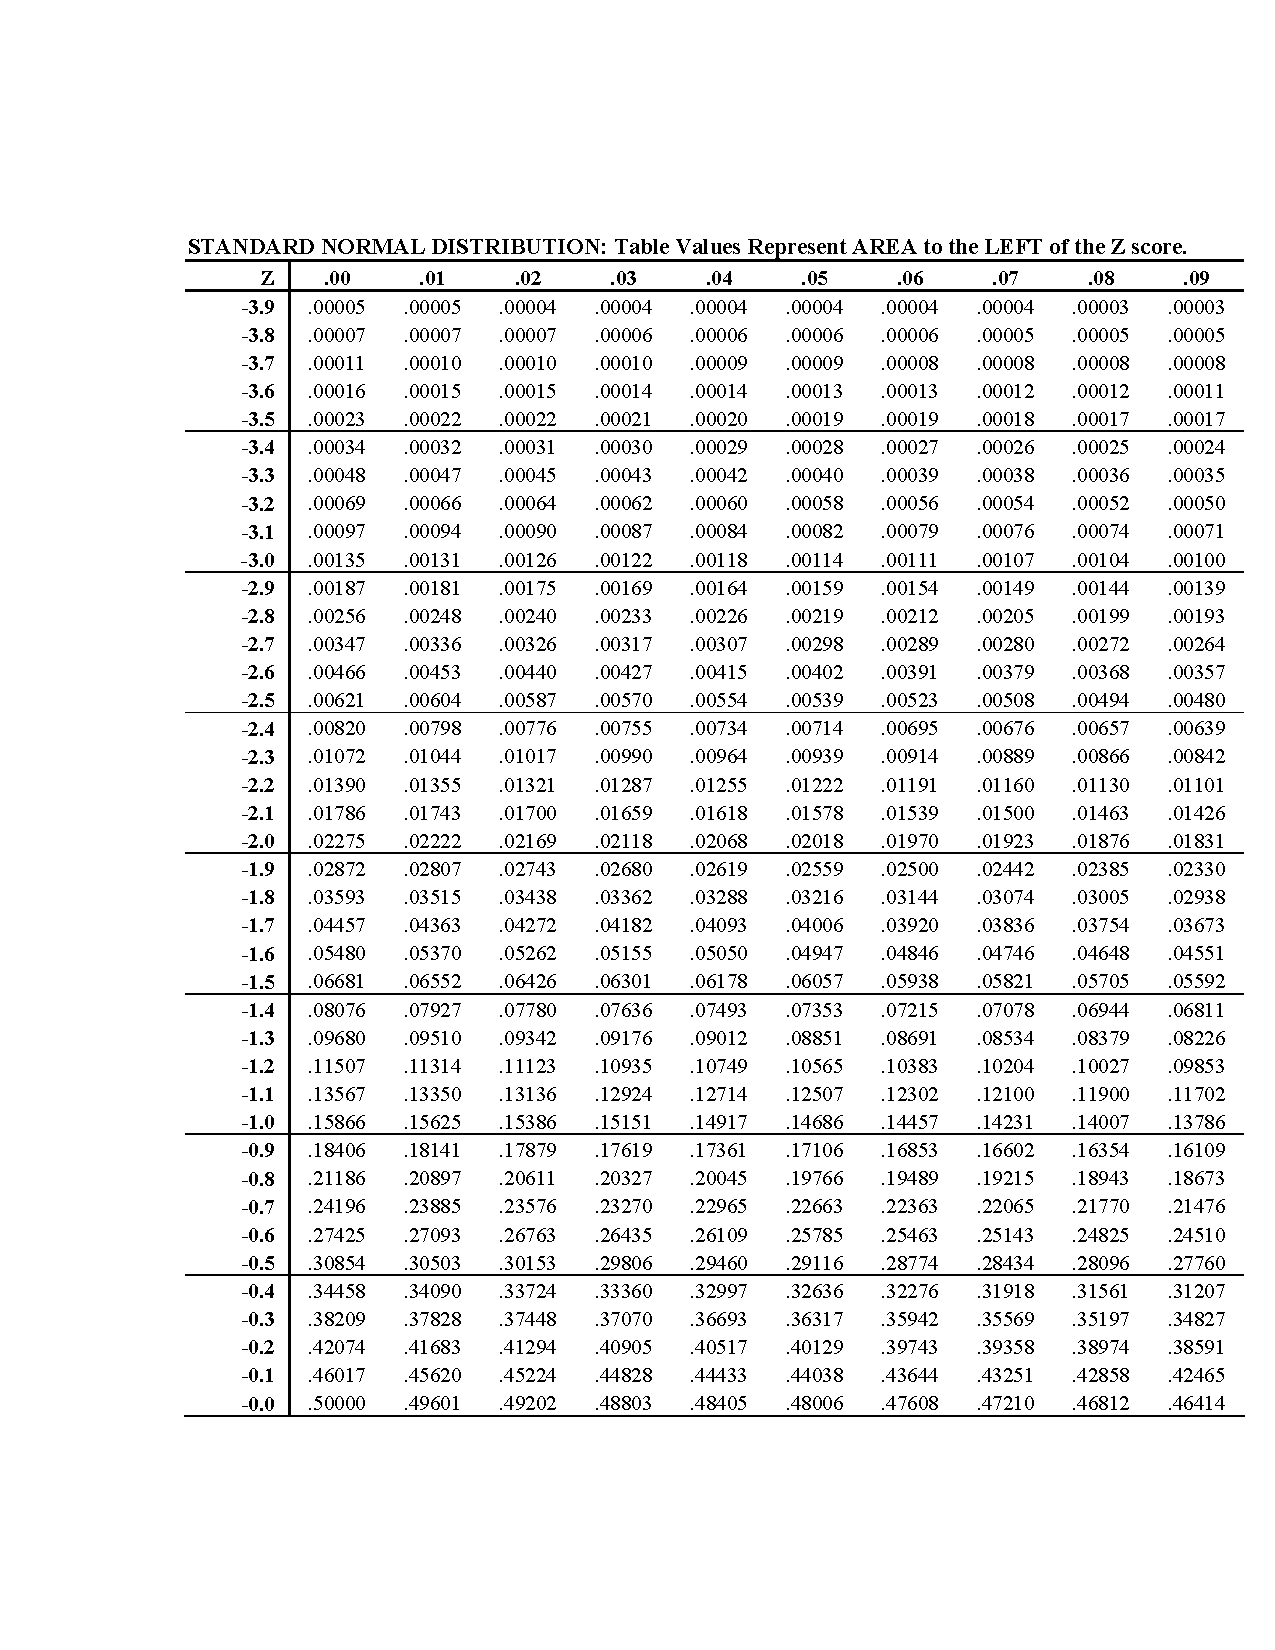
\includegraphics[page=1, width=0.9\linewidth, trim=4cm 4cm 1.25cm 4cm]{standardnormaltable.pdf}
%     \label{zscore}
% \end{figure}

% \begin{figure}[!ht]
%     \centering
%     \includegraphics[page=2, width=0.9\linewidth, trim=4.1cm 4cm 1.15cm 4cm]{standardnormaltable.pdf}
% \end{figure}

\subsection{Sampling Distributions}

\subsubsection{Unknown Variables}
Parameters: measures that describe populations \\
Statistics: measures that describe samples \\
Sampling distribution: distribution of a statistic across all possible samples

\subsubsection{Estimators and Bias}
Estimator: see Section~\ref{sec:confidence_intervals} for definition.
\begin{gather}
    \text{Bias}(W) = \text{E}(W)-\theta \\
    \text{Variability} \propto \frac{1}{\text{sample size}}
\end{gather}
where $W$ is the estimator and $\theta$ is the parameter. \\[0.5cm]
Unbiased estimator: mean of sampling distribution is equal to value of parameter. For example, sample mean is an unbiased estimator because the mean of the sampling distribution of sample means is equal to the value of the parameter.

\subsubsection{Sample Means}
\begin{gather}
    \mu_{\bar{x}}=\mu \\
    \sigma_{\bar{x}}=\frac{\sigma}{\sqrt{n}}
\end{gather}
where $\bar{x}$ is the sampling distribution and $\mu$ is the mean of the population. Thus, sampling distributions have no bias. \\[0.5cm]
Central Limit Theorem: sampling distribution of the mean is approximately normal for any distribution.

\subsection{Confidence Intervals}
\label{sec:confidence_intervals}
\begin{enumerate}
    \item Point estimator: estimate of a population parameter
    \item Point estimate: value of statistic for a sample
    \item Confidence level C: the percent probability that a random sample interval will capture parameter value; in C$\%$ of all samples, the sample interval will include parameter value
    \item Confidence interval: point estimate $\pm$ margin of error; range of plausible values for parameter value
\end{enumerate}

\subsubsection{Margin of Error}
Purpose: addresses sample variability
\begin{gather}
    CI = \bar{x} \pm c_{\alpha/2}*\text{se}(\bar{x}) \\
    \text{se}(\bar{x}) = \frac{s}{\sqrt{n}}
\end{gather}
where $c_{\alpha/2}$ is the critical value (the number of standard errors the interval includes), obtained from the t-table (Figure~\ref{fig:t_table}).

\begin{gather}
    \text{confidence level} \propto CI \\
    CI \propto \frac{1}{\text{sample size}}
\end{gather}
Note: 95\% confident does not mean 95\% chance that true mean is in interval; rather, if data collection was done 100 times, 95 times the interval would contain the true mean. Confidence does not equate to chance.

\subsubsection{T-Table}
\begin{figure}[!ht]
    \centering
    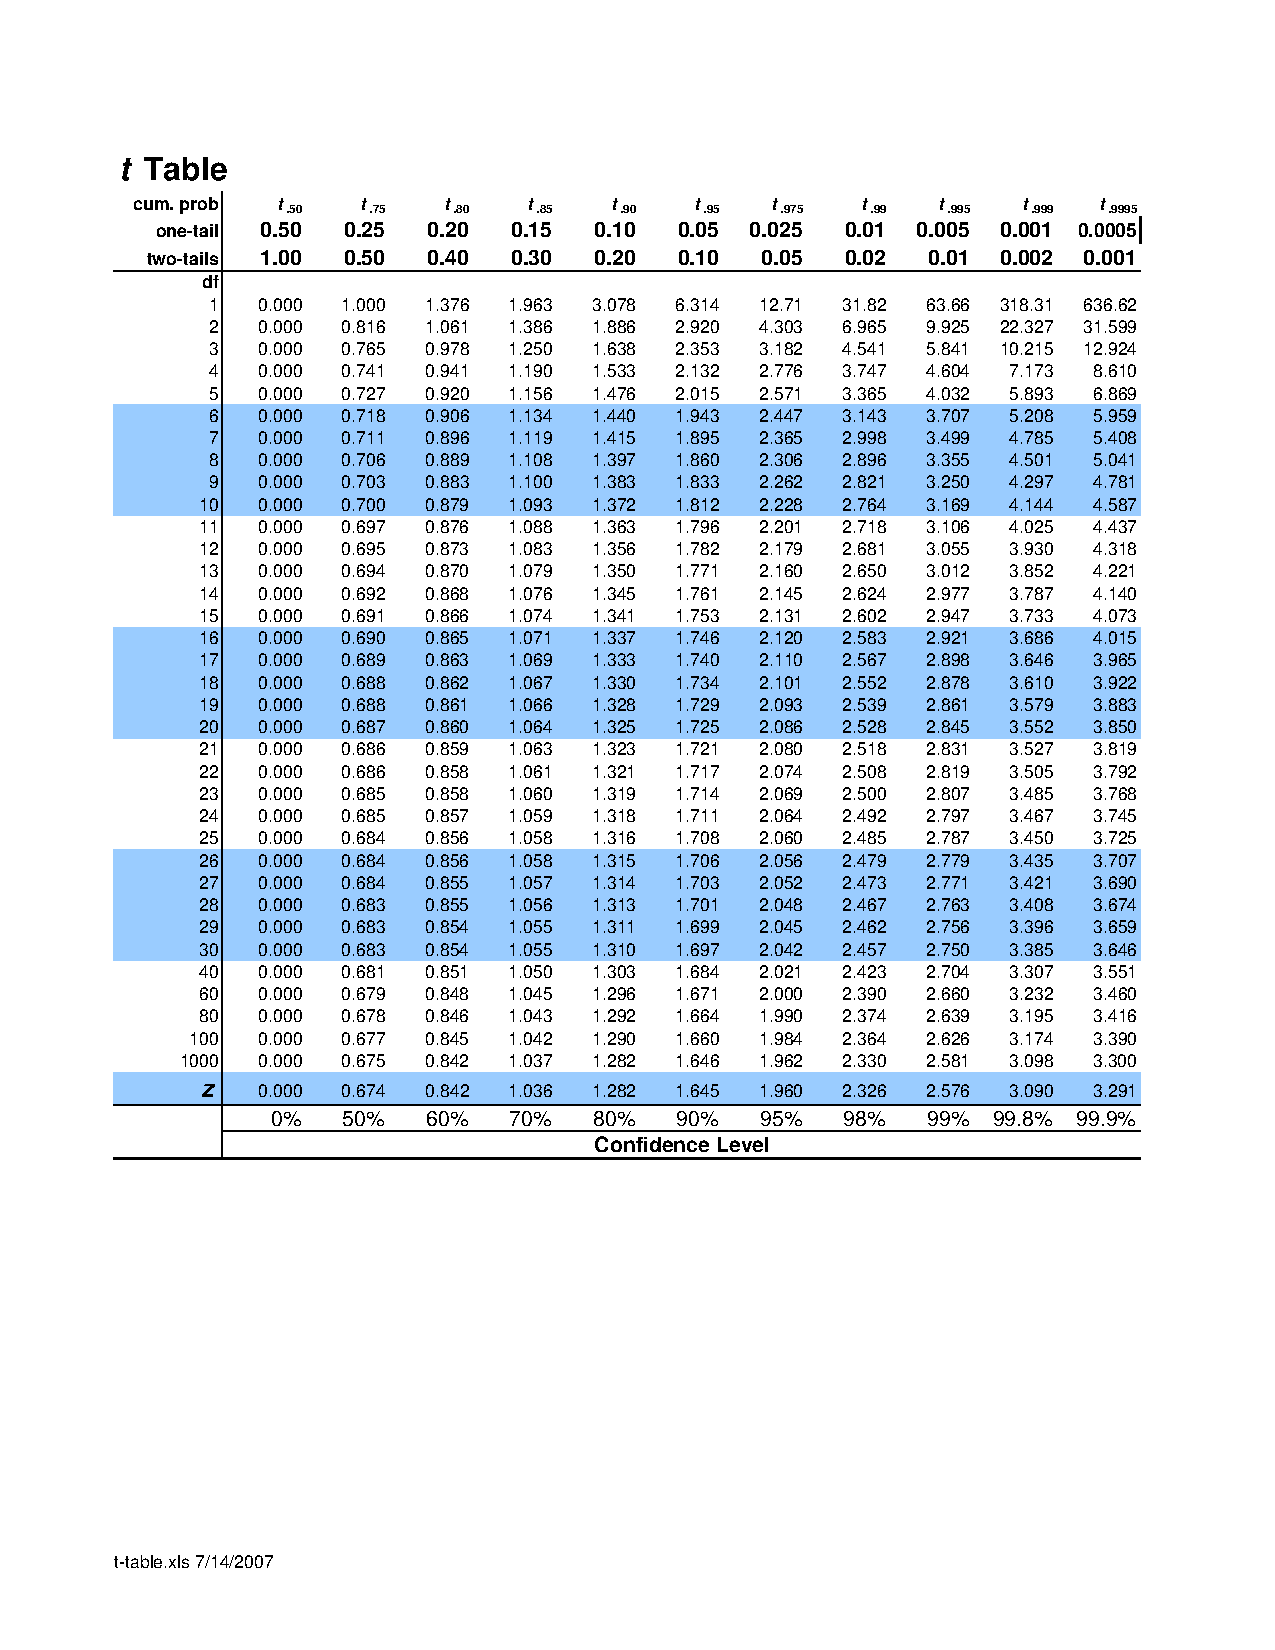
\includegraphics[width=\linewidth, clip, trim=2cm 8cm 2cm 2.5cm]{t-table.pdf}
    \label{fig:t_table}
\end{figure}

\subsubsection{Computation}
Preconditions:
\begin{enumerate}
    \item Random sample selection
    \item $<$10\% of population
    \item Sufficient sample size ($>$30)
\end{enumerate}

\noindent Steps:
\begin{enumerate}
    \item Calculate mean
    \item Find margin of error
    \item Find range of sample interval
    \item Interpret in context
\end{enumerate}

\section{Other}
\begin{enumerate}
    \item reduce space between enumerate items
\end{enumerate}

\noindent \begin{flushright} \hyperref[sec:top]{back to top} \end{flushright}
\end{document}